\documentclass[10pt,twocolumn,letterpaper]{article}
\usepackage[margin=0.75in]{geometry}
\usepackage{amsmath}
\usepackage{graphicx}
\usepackage{microtype}
\usepackage[T1]{fontenc}
\usepackage{newtxtext,newtxmath}
\usepackage{pgfplots}
\pgfplotsset{compat=1.18}
\title{Selective Identity Reconnection in Online\\ Multi-Object Tracking}
\author{}
\date{}

\begin{document}

\makeatletter
\twocolumn[{
\begin{@twocolumnfalse}
\maketitle
\vspace{-1.2em}
\begin{abstract}
\noindent An online tracker that recovers a lost person must decide whether
the return belongs to the old identity, and a wrong decision is silent: the
wrong person inherits the identifier and every later frame follows. We treat
reactivation as a decision and place a scalar gate in front of it. The gate
reads detector confidence, track state, and the margins between the proposed
assignment and its competitors; it uses no appearance descriptor, so it
applies where only a detection model and a geometric tracker exist.
Thresholds are fixed on calibration sources before any test source is read.
On the official PersonPath22 test subset, with admission counts matched
across methods, the gate fails in 98 of 381 evaluated reactivations against
158 of 390 for the native association cost, and fails less often than the
association score of a published tracker ported into the same host, by 9.72
to 13.50 percentage points. The gain comes from product terms between gap
length and motion or ambiguity evidence, and holds at one of five operating
points. The cost is 136 fewer recovered gaps and 1.65 fewer HOTA points than
an unconstrained tracker.

\vspace{0.4em}
\noindent\textbf{Keywords:} multi-object tracking; identity reconnection;
association gating; track recovery; operating-point selection
\end{abstract}
\vspace{1.4em}
\end{@twocolumnfalse}
}]
\makeatother

\section{Introduction}

A tracker that has lost a person and finds them again must decide whether
the return belongs to the old identity. ByteTrack
\cite{zhang2022bytetrack} keeps a lost track alive for thirty frames and
re-attaches any later detection that clears its association threshold.
When the decision is right, an identity survives an occlusion and the
trajectory continues. When it is wrong, nothing announces the error: the
wrong person inherits the identifier, every later frame is attached to
that identifier, and every count, dwell time or trajectory built on top of
it is wrong from that moment on. Reconnection failures are silent, which
is why they deserve more attention than their share of association events
would suggest.

Work on the problem takes two forms. One improves the association cost
itself, through motion models, matching cascades and observation-centric
updates \cite{zhang2022bytetrack,aharon2022botsort,cao2023ocsort}. The
other adds appearance, either as a re-identification branch inside the
tracker or as a linking stage after it. We ask a narrower question that
neither answers directly. Given the proposals a tracker has already made,
which ones should be committed?

Three deployment settings make that narrow question worth asking. A
privacy-constrained installation may not permit storing face or clothing
embeddings at all. An edge device may not have the budget to run a second
network beside the detector. A retrospective analysis may inherit a tracker
whose association rule cannot be changed, only wrapped. In each case the
available lever is not a better match but a better decision about whether to
commit the match, and in each case the decision has to be made from the
evidence at that frame.

We treat reactivation as a decision and place a scalar gate in front of
it. The gate reads the detector confidence, the predicted box residuals,
the track age, the observed gap, and the margins between the proposed
assignment and its best competitors in the same row and column. A
regularized logistic score combines these, and product terms let the
weight of motion agreement and of assignment ambiguity change with gap
length. A refused detection returns to the tracker as unmatched, so the
decision changes the state that later frames see. No appearance network is
trained and no gallery is stored: the gate decides from geometry.

The paper makes four claims. \textbf{First, the effect survives matched
admission counts.} Counting failures rewards silence, so we re-select
thresholds until the native association cost, an additive score and the
interaction score admit the same number of actions per source. At the cap
of twelve admissions per source, ByteTrack then fails in 98 of 381
evaluated reactivations against 158 of 390 for its native cost, and
verified-correct reactivations rise from 232 to 283. \textbf{Second, the
comparison is against a published score, not only a hand-set threshold.}
After porting the BoostTrack association similarity into the same host and
checking the port element by element, the interaction score fails less
often in all five operating points we tested, by 9.72 to 13.50 percentage
points. \textbf{Third, the gain comes from the product terms and not from
extra summaries of the competing assignments}: a score that drops the
products and keeps only the three summaries has no contrast interval that
excludes zero at any of the five operating points, while the full score
lowers the failure proportion by 3.29 points at the point where the effect
is established. \textbf{Fourth, the cost is
explicit.} Relative to an unconstrained ByteTrack the gate removes 1,397
evaluated failures and 136 natural gaps, and HOTA falls by 1.65 points. We
report that as the price of the decision rather than argue it away.

One boundary applies throughout. The gate uses no appearance signal, so
the claim covers detection-only pipelines; and every failure proportion in
this paper is an observation on the split that names it, not a bound on
unseen sources.

\section{Related Work}

\subsection{Association and reactivation in online trackers}

Tracking-by-detection pipelines pair a detector with a data association
rule. SORT \cite{bewley2016sort} fixed the modern form: a Kalman filter
predicts each track, and a Hungarian assignment on box overlap consumes
the detections. DeepSORT \cite{wojke2017deepsort} added an appearance
metric to the same cascade. ByteTrack \cite{zhang2022bytetrack} broke the
rule that low-confidence detections are discarded, and it introduced the
track buffer that makes reactivation routine: a track survives thirty
frames of absence and any later detection above the association threshold
is re-attached. BoT-SORT \cite{aharon2022botsort} improved the motion model
and compensated camera movement; OC-SORT \cite{cao2023ocsort} replaced the
filter state used in matching with observation-centered estimates.

These systems change what counts as a good match. Reconnection is a
by-product of that choice: the tracker keeps a lost track alive, and
whatever clears the threshold is accepted. The buffer length and the
threshold decide how often this happens, and neither is a statement about
whether a particular return is the same person. That is the gap we
address.

In a two-stage cascade the reactivation decision is made by the same scalar
threshold that governs ordinary association. That threshold is tuned for
the bulk of assignments, most of which involve no gap at all, so a return
after eight frames and a return after one frame are judged by the same
number; the only per-event variation comes from whatever motion cost the
filter happened to predict. Nothing in the cascade asks whether the
evidence at this particular proposal is strong. A learned per-proposal
score asks exactly that.

\subsection{Appearance-based re-identification}

The standard answer to an ambiguous return is an appearance descriptor.
DeepSORT \cite{wojke2017deepsort} introduced the idea, and later trackers
keep a re-identification branch alongside motion, or link tracklets after
tracking with a learned similarity. Where a trained embedding model and
enough pixels per crop are available, this signal is strong, and it
addresses occlusion gaps that geometry cannot resolve.

A descriptor is not free of failure modes of its own. Clothing changes,
matching uniforms and crowds of near-identical people all degrade it, and a
gallery has to be maintained across the sequence rather than read once. Its
cost also scales with the number of active tracks instead of the number of
reactivations, which matters in long sequences where most tracks live for a
few seconds.

It also imposes conditions we do not assume. It requires a network, a
feature gallery or a re-identification budget, and crops of usable
resolution at both ends of the gap. On sparse annotation grids and on
small or heavily occluded boxes those conditions often fail together. We
therefore restrict the study to detection-only evidence and treat
appearance as the natural extension rather than a missing component. The
comparison we do make is against an association score from a published
tracker, BoostTrack \cite{stanjoevic2024boosttrack}, ported into the same
host so that only the scoring component changes.

\subsection{Selection and risk control}

Gating proposals is a selection problem: a threshold is chosen from data,
and the chosen threshold's measured risk is optimistic by construction.
Learn-then-test \cite{angelopoulos2021learn} calibrates this choice over a
family of policies and returns a valid risk level. Closely related work
bounds the coverage of candidate transition sets in tracking
\cite{li2022pac} and propagates detector-box uncertainty through the
tracking pipeline \cite{su2024motcup}. We use the vocabulary of that line
of work to describe
what our selection rule does, and we report the selected policies'
observed failure proportions without claiming a calibrated bound. What
distinguishes the present study is not the statistics but the object being
measured: committed reactivations after closed-loop replay, counted
separately from the gap recoveries they produce.

Selection and filtering are easy to conflate, and the difference decides
what a fair comparison looks like. A threshold selects one operating point
for every proposal; a score decides each proposal on its own evidence. Two
rules that admit the same total number of actions can still commit
different actions, so a comparison that matches only the totals still
leaves the per-proposal decision unexamined. That is why we match admission
counts source by source and compare the paired decisions rather than the
aggregate rate alone.

\subsection{Benchmarks and how tracking is scored}

Three benchmarks shape what a tracking result is allowed to claim. MOT16
\cite{milan2016mot16} standardised annotation and made crowded pedestrian
sequences the default test, where clothing and build vary enough that an
appearance model has something to learn. DanceTrack
\cite{sun2022dancetrack} removes that advantage by design: its dancers wear
near-identical costumes, so appearance carries almost no information and
association has to rest on motion. PersonPath22
\cite{shuai2022personpath22}, the dataset used here, sits elsewhere again,
with sparse manual keyframes, a frozen detector and long sequences in which
the same person leaves the frame and comes back.

Metrics moved with the benchmarks. HOTA \cite{luiten2021hota} separates
detection accuracy from association accuracy and reports both before
combining them, which matters when a method changes only the association
step. PersonPath22 supports a measurement that neither benchmark offers
directly: because each keyframe carries both a box and an identity, a
detector gap can be located exactly, and its recovery counted separately
from the association quality of the sequence as a whole. That separation is
what lets this paper report an action-level failure proportion next to a
trajectory-level score instead of choosing between them.

\section{Selective track reactivation}

A tracker that loses a person and finds them again has to decide whether
the return belongs to the old identity. Accept, and the track continues;
refuse, and the detection re-enters the association pool, changing every
proposal that follows. We place a scalar gate in front of that commitment.
The gate reads the detector output and the track state and nothing else:
no appearance network, no gallery, no future frames. That restriction is
what lets the method run where only a detector and a geometric tracker
are available.

Let $x$ record the detector confidence, the predicted box residuals, the
track age and the observed gap, and the costs of the competing one-to-one
assignments at the frame where the reactivation is proposed. Write $m_r$
and $m_c$ for the best admissible competitor cost minus the chosen cost in
the same row or column of the assignment matrix, and use
$m=\min(m_r,m_c)$ for the weaker side. Base transformations $z(x)$ are
formed first, the interaction vector second, and its coordinates are
standardized before fitting
\begin{align*}
g(x) &= b+w^\top \phi(x),\\
\phi(x) &= [z(x),\,m,\,|m_r-m_c|,\,h d,\,h o,\,h m,\,q m,\ldots].
\end{align*}
Here $h$ is the transformed elapsed gap, $d$ and $o$ the normalized center
difference and box overlap, and $q$ the detection confidence. The product
terms let the weight of motion agreement and of assignment ambiguity move
with gap length, which a purely additive score cannot express.
We fit $g$ with regularized logistic loss on annotated development
proposals. An ablation adds a within-source ranking loss
$\log(1+\exp(g_{\rm incorrect}-g_{\rm correct}))$.
A threshold on $g$ governs reactivation. A refused detection returns to
the tracker as unmatched, so the next association step sees the state that
decision produced.

\subsection{Fixing the operating point}

A gate is only meaningful if its threshold is fixed before evaluation.
Candidates are drawn from development score quantiles and, where the
quantile grid cannot match methods, from a denser $0.35$--$0.97$ sweep in
steps of $0.01$. Every candidate is replayed on the calibration sources,
and the operating point is the one that recovers the most gaps while its
calibration failure proportion stays under a ceiling. We report a relaxed
and a strict ceiling: a single number would hide the shape of the
trade-off. Thresholds and their input hashes are written out before any
test source is read.

The procedure is a selection, and we treat it as one. A sweep scores up to
63 thresholds, and taking the best of them on the data that also set the
ceiling tilts the resulting risk downward. Learn-then-test calibrates this
kind of choice over a policy family \cite{angelopoulos2021learn}, and
guarantees exist for candidate-set coverage \cite{li2022pac} and for
detector uncertainty \cite{su2024motcup}; we do not apply them here. Every
failure proportion in what follows is an observation on the named split,
not a bound on unseen sources.

\section{Experiments}

\subsection{Data and evaluation}
We study reconnection on PersonPath22 \cite{shuai2022personpath22}, using
its native manual keyframes and the publisher's FCOS person detections
trained on CrowdHuman, aligned frame by frame with the annotated sources.
The observation grid is nominally 5~Hz. Of the 236 public clips we assign
16 publisher-hosted training assets to development, 91 to calibration, and
hold out 74 publisher-hosted official test assets; the 55 clips carrying
external source mappings stay out of this protocol. Detector input,
matching rules and evaluation sequences are identical for every tracker
variant.

The setting is deliberately detection-only. No re-identification network
is trained and no gallery is stored: the gate must decide from geometry,
detector confidence and association margins alone. Appearance
re-identification, as in the ReID variant of BoT-SORT
\cite{aharon2022botsort}, carries an orthogonal and often stronger signal
and is the natural next comparison rather than a component of this one.

To measure detector-gap recovery, we first matched detection boxes and
ground-truth persons one to one at IoU $\geq 0.50$. For each ground-truth
identity, a gap consisted of one to five intervening annotated keyframes
with no matched detection. We counted a recovery if the track identifier
at the first returned detection matched its identifier before the gap. We
used the same ground-truth/detector gap list for all policies and included
cases without an emitted pre-gap identity in the denominator.

We also audited the tracker's reactivation actions separately from gap
recovery. A reactivation was correct if the specified one-to-one matching
assigned its previous emitted track and its new detector box to the same
annotated person; otherwise it was counted as wrong or unverifiable,
except where an unmatched endpoint overlapped an annotated ignore region
by more than half its own box area. Ignored actions are reported
separately. The audit runs after tracking, so the gate itself never sees
an annotation. Overall metrics were HOTA, AssA, IDF1 and ID switches,
computed with TrackEval on the native keyframe grid
\cite{luiten2021hota}, with PersonPath22's distractor and crowd treatment.

\subsection{Comparison and model fitting}
We replayed ByteTrack \cite{zhang2022bytetrack} and a motion-only BoT-SORT
configuration \cite{aharon2022botsort}, each from frame one, with the gate
deciding on every native old-ID reactivation before the tracker updated
its state. We compared the unrestricted tracker, a source cap alone, a
threshold on the native association cost, a threshold on the nearest
competitor margin, an additive linear score, the interaction score, and
the interaction score with the within-source ranking term. Capped policies
admit at most 12 actions per source, and ignored admissions count against
the cap as well. Scores were fit on the development sources for 200
Adam updates (learning rate 0.04, coefficient penalty 0.002) on a GeForce
RTX 3060 Ti. Candidate thresholds came from development score quantiles
fixed before calibration. For each score we take the operating point that
recovers the most gaps within a common empirical calibration ceiling while
keeping at least 20\% of calibration sources active, then run the selected
policies on the official test assets without tuning.

\subsection{Official split results}
The official test subset contained 9,320 keyframes and 3,155 eligible
detector gaps. At a common empirical calibration ceiling of 47.23\%, the
ByteTrack interaction gate reduced the tested incorrect or unverifiable
action proportion from 46.77\% to 35.39\% relative to the native
association threshold, and raised verified correct reactivations from 239
to 283 while using 438 evaluated admissions instead of 449. Gap recoveries
were 393 and 388. The paired source resampling interval was
$[-16.57,-6.40]$ percentage points for the failure-rate difference and
$[-0.33,0.67]$ for gap recovery (10,000 replicates). The interaction score
also reduced the failure proportion against the cap-only and linear
controls at this ceiling.

At the 20\% calibration ceiling both ByteTrack scores recovered 383 gaps,
with observed failure proportions of 21.24\% for the interaction score and
21.15\% for the linear score. On motion-only BoT-SORT the interaction
score recovered 334 gaps against 327 for the linear score, with 16.19\%
versus 18.31\% checked failures. The paired intervals were $[0.05,0.48]$
percentage points for gap recovery and $[-4.94,0.75]$ for the failure
proportion. At the relaxed BoT-SORT ceiling of 42.15\% the linear score
had the lower observed failure, 25.19\% against 37.28\%. The added
pairwise ranking loss produced no consistent benefit.

\begin{figure*}[t]
\centering
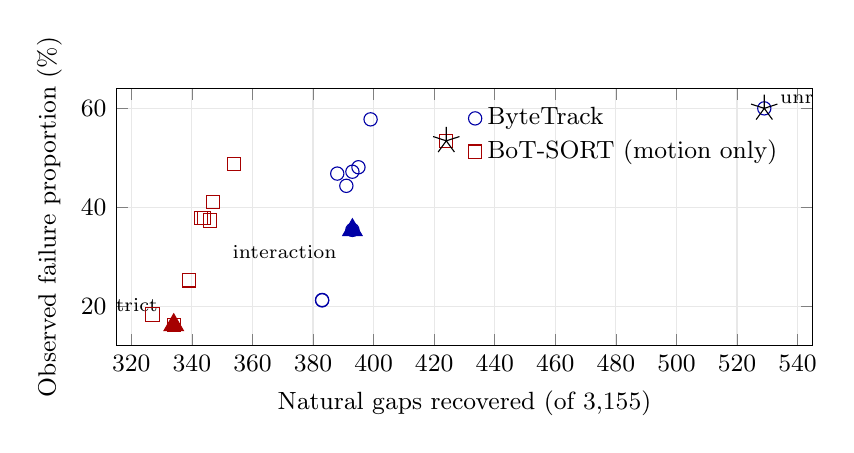
\begin{tikzpicture}
\begin{axis}[
    width=0.86\textwidth,
    height=0.40\textwidth,
    xlabel={Natural gaps recovered (of 3,155)},
    ylabel={Observed failure proportion (\%)},
    xmin=315, xmax=545,
    ymin=12, ymax=64,
    grid=major,
    grid style={gray!18},
    legend pos=north east,
    legend cell align=left,
    legend style={draw=none, fill=none, font=\small},
    tick label style={font=\small},
    label style={font=\small},
    mark size=2.4pt,
]
\addplot[only marks, mark=o, mark options={solid}, color=blue!65!black,
         forget plot] coordinates {
    (529,59.95) (399,57.73) (388,46.77) (391,44.30) (395,48.05)
    (393,35.39) (393,47.15) (383,21.15) (383,21.24)
};
\addlegendimage{only marks, mark=o, color=blue!65!black}
\addlegendentry{ByteTrack}
\addplot[only marks, mark=square, mark options={solid}, color=red!65!black,
         forget plot] coordinates {
    (424,53.39) (354,48.69) (343,37.76) (347,41.02) (339,25.19)
    (346,37.28) (344,37.78) (327,18.31) (334,16.19)
};
\addlegendimage{only marks, mark=square, color=red!65!black}
\addlegendentry{BoT-SORT (motion only)}
\addplot[only marks, mark=star, mark size=5pt, color=black] coordinates {(529,59.95)};
\addplot[only marks, mark=star, mark size=5pt, color=black] coordinates {(424,53.39)};
\addplot[only marks, mark=triangle*, mark size=4pt, color=blue!65!black] coordinates {(393,35.39)};
\addplot[only marks, mark=triangle*, mark size=4pt, color=red!65!black] coordinates {(334,16.19)};
\node[font=\scriptsize, anchor=south west] at (axis cs:531,59.0) {unrestricted};
\node[font=\scriptsize, anchor=north east] at (axis cs:391,34.2) {interaction};
\node[font=\scriptsize, anchor=south east] at (axis cs:332,16.9) {strict};
\end{axis}
\end{tikzpicture}
\caption{Every evaluated policy on the official PersonPath22 test subset,
plotted by the number of natural gaps it recovers and the observed
proportion of failed evaluated reactivations. Stars mark the unconstrained
trackers, triangles the relaxed interaction gate, and the lower-left
cluster the strict ceilings. Policies to the right of a given point recover
more gaps; policies below it fail less often. The frontier runs from the
strict ceilings at the lower left to the unconstrained tracker at the upper
right, so no single policy is best on both axes.}
\label{fig:tradeoff}
\end{figure*}


\begin{table*}[t]
\centering
\small
\caption{PersonPath22 native-keyframe official-test subset. Gap recovery
uses the same 3,155 gaps for every policy. Admits and fails exclude
ignored actions. HOTA, AssA and IDF1 are on a 0--100 scale; IDSW is a
count; Risk is the observed failure proportion. The cap-only gate applies
the same source cap. Rows without a strict marker use the relaxed
calibration ceiling. Section~\ref{sec:matched} re-selects thresholds under
a matched-acceptance rule, so its counts differ from these.}
\label{tab:reconnection-main}
\begin{tabular}{llrrrrrrrr}
\hline
Tracker & Reactivation policy & Gaps kept & Admits & Fails & Risk (\%) & HOTA & AssA & IDF1 & IDSW \\
\hline
OC-SORT & External reference & 174 & -- & -- & -- & 41.83 & 41.22 & 52.15 & 3790 \\
\hline
ByteTrack & Unrestricted & 529 & 2589 & 1552 & 59.95 & 46.64 & 42.33 & 56.73 & 6662 \\
 & Cap only & 399 & 537 & 310 & 57.73 & 44.69 & 39.32 & 52.94 & 7129 \\
 & Native cost & 388 & 449 & 210 & 46.77 & 44.76 & 39.41 & 53.16 & 7104 \\
 & Nearest margin & 391 & 456 & 202 & 44.30 & 44.84 & 39.57 & 53.14 & 7132 \\
 & Linear & 395 & 514 & 247 & 48.05 & 44.90 & 39.63 & 53.38 & 7131 \\
 & Interaction & 393 & 438 & 155 & 35.39 & 44.99 & 39.81 & 53.38 & 7022 \\
 & Interaction + ranking & 393 & 509 & 240 & 47.15 & 44.91 & 39.69 & 53.34 & 7131 \\
 & Linear (strict) & 383 & 331 & 70 & 21.15 & 44.87 & 39.63 & 53.25 & 7120 \\
 & Interaction (strict) & 383 & 339 & 72 & 21.24 & 44.87 & 39.63 & 53.23 & 7116 \\
\hline
BoT-SORT & Unrestricted & 424 & 1858 & 992 & 53.39 & 46.84 & 43.78 & 56.57 & 5909 \\
(motion only) & Cap only & 354 & 495 & 241 & 48.69 & 45.04 & 40.71 & 53.03 & 6616 \\
 & Native cost & 343 & 392 & 148 & 37.76 & 44.99 & 40.67 & 52.98 & 6656 \\
 & Nearest margin & 347 & 451 & 185 & 41.02 & 45.10 & 40.83 & 53.07 & 6654 \\
 & Linear & 339 & 397 & 100 & 25.19 & 45.20 & 40.99 & 53.29 & 6603 \\
 & Interaction & 346 & 448 & 167 & 37.28 & 45.14 & 40.88 & 53.20 & 6566 \\
 & Interaction + ranking & 344 & 450 & 170 & 37.78 & 45.14 & 40.87 & 53.16 & 6611 \\
 & Linear (strict) & 327 & 284 & 52 & 18.31 & 45.05 & 40.83 & 53.05 & 6628 \\
 & Interaction (strict) & 334 & 278 & 45 & 16.19 & 45.06 & 40.85 & 53.02 & 6626 \\
\hline
\end{tabular}
\end{table*}

The unrestricted trackers retain more natural gaps and higher overall
HOTA (Table~\ref{tab:reconnection-main}). Relative to unrestricted
ByteTrack, the relaxed interaction gate removes 1,397 evaluated failures
and 136 natural gaps, and HOTA falls by 1.65 points. That is the price of
selective admission, and we state it as a price rather than argue it away:
the gate buys decision reliability, not a better tracker. OC-SORT
\cite{cao2023ocsort} appears as an overall tracking reference whose output
supports the same gap evaluation, although its internal reactivation
mechanism follows a different protocol.

\subsection{Matched acceptance}
\label{sec:matched}

Counting failures rewards silence. A gate that admits nothing has no
failures, and Table~\ref{tab:reconnection-main} compares policies that
admit anywhere from 278 to 2,589 actions, so part of its ordering reflects
admission count rather than decision quality. We remove that confound
directly: for each tracker and each cap $B\in\{6,12,24\}$ we re-select
thresholds so that the native association cost, the additive score and the
interaction score admit the same number of actions per source.

Matching is not free. The target is the calibration admission count per
source, and a method may deviate by 0.10 admissions per source or 5\% of
the target, whichever is larger. None of the 18 cells of the original
quantile grid cleared that bar, so the sweep was densified to steps of
0.01 and replayed on calibration until 17 operating points could be
locked. Seven of them
still satisfied the between-method tolerance on the test sources; the
other ten are reported as sensitivity results. In all 17, at least one
method ends further from its calibration target than the tolerance allows,
so these are comparisons between methods, not reproductions of a fixed
admission rate.

Against the native association cost the interaction score had the lower
failure proportion at all 17 points, by 8.70 to 23.00 percentage points,
with every per-comparison interval below zero. At the cap of 12 and the
high ceiling the gap is concrete: ByteTrack fails in 98 of 381 evaluated
admissions against 158 of 390, and motion-only BoT-SORT in 81 of 367
against 116 of 350, with paired intervals of $[-20.95,-8.80]$ and
$[-17.29,-5.15]$ points. Gap recovery moves by $+0.41$ $[+0.03,+0.84]$
and $+0.10$ $[-0.35,+0.60]$ points. The reliability gain therefore does
not cost recovery at this operating point, and it is not an artefact of
admitting less.

Against the additive score the picture is thinner. Two of the 17 contrasts
have an interval entirely below zero -- $-3.29$ $[-5.37,-1.10]$ at the
ByteTrack high point and $-2.57$ $[-5.05,-0.16]$ for BoT-SORT at $B=24$ --
and the remaining 15 cross zero, several with a positive point estimate
($+1.54$ $[-1.83,+4.85]$ at the ByteTrack mid point). Matching admission
counts separates the interaction score from the native cost cleanly and
from an additive model only at some operating points. We keep that
distinction instead of averaging over it.

\subsection{Where the gain comes from}
\label{sec:ablation}

Two questions decide whether the score is a contribution or a fitted
artefact: which part of $\phi$ carries the effect, and whether a published
association score does the same job more simply.

For the first we build three scores on identical development proposals,
labels and sample order. The 12-dimensional and the full 23-dimensional
scores reuse their locked weights. The 15-dimensional score keeps the 12
base features and adds three competition summaries -- the minimum margin,
the absolute difference of the margins, and the largest transformed
alternative count -- and is refitted from scratch, since truncating the
full model's weights cannot separate the two hypotheses. Fitting uses the
original settings, including an explicit ranking weight of zero. The
15-dimensional feature prefix is verified to equal the first 15 entries of
the full vector on the same proposal, and the reloaded 12- and
23-dimensional configurations reproduce their stored scores.

Table~\ref{tab:round3} gives the paired contrasts. Adding the eight product
terms to the 15-dimensional score lowers the failure proportion by 3.29
points at the ByteTrack high point, interval $[-5.82,-0.92]$. At the mid
point the difference reverses to $+1.60$ $[-1.43,+4.48]$, and all three
BoT-SORT intervals cross zero. The three competition summaries alone
produce no contrast whose interval excludes zero at any of the five
points. The effect belongs to the group of product terms as a whole, and
it is established at one operating point rather than throughout.

For the second question we port the association similarity of the published
BoostTrack tracker \cite{stanjoevic2024boosttrack} into the same role. The
host tracker assigns exactly as
before; for the proposals it has already made, we read the BoostTrack
similarity of the proposed pair from the current-frame candidates and the
host track state, then apply the same gate and the same handling of
refused detections. Detection boxes, scores, native assignments, motion
updates and later stages are untouched. A switched scoring component can
otherwise be confused with a change of input, so the port is checked
numerically first: on 1,747 development candidate matrices the ported and
the authors' function agree to a maximum absolute difference of zero
across 745,096 elements, and for motion-only BoT-SORT, whose state stores
width and height rather than height and aspect ratio, 420,620 elements
agree to zero with the covariance propagated by a first-order
approximation.

\begin{table*}[t]
\centering
\small
\caption{Interaction ablation and external score, cap of 12 admissions per
source. Each row is one paired contrast over the same 74 sources,
resampled 10,000 times (seed 362). Fails/admits counts evaluated decisions
after ignore-region removal and is not the gap-recovery denominator.
$\Delta$ is the left policy's failure proportion minus the right policy's,
in percentage points; negative favours the left policy. BoostTrack rows
compare the ported association score inside the same host.}
\label{tab:round3}
\begin{tabular}{lllrrr}
\hline
Tracker & Ceiling & Contrast & Fails/admits (L / R) & $\Delta$ (pp) & 95\% CI \\
\hline
ByteTrack & high & 23 vs 15 & 98/381 \;/\; 112/386 & $-3.29$ & $[-5.82,-0.92]$ \\
 & mid & 23 vs 15 & 69/327 \;/\; 62/318 & $+1.60$ & $[-1.43,+4.48]$ \\
 & high & 23 vs BoostTrack & 98/381 \;/\; 152/388 & $-13.45$ & $[-19.06,-8.06]$ \\
 & mid & 23 vs BoostTrack & 69/327 \;/\; 109/315 & $-13.50$ & $[-18.88,-8.40]$ \\
\hline
BoT-SORT & low & 23 vs 15 & 30/222 \;/\; 33/225 & $-1.15$ & $[-3.02,+0.46]$ \\
(motion) & mid & 23 vs 15 & 57/293 \;/\; 54/291 & $+0.90$ & $[-1.56,+3.54]$ \\
 & high & 23 vs 15 & 81/367 \;/\; 81/359 & $-0.49$ & $[-2.46,+1.40]$ \\
 & low & 23 vs BoostTrack & 30/222 \;/\; 53/214 & $-11.25$ & $[-17.32,-5.32]$ \\
 & mid & 23 vs BoostTrack & 57/293 \;/\; 83/273 & $-10.95$ & $[-18.09,-3.84]$ \\
 & high & 23 vs BoostTrack & 81/367 \;/\; 110/346 & $-9.72$ & $[-16.00,-3.66]$ \\
\hline
\end{tabular}
\end{table*}

The interaction score fails less often than the ported score in all five
contrasts, by 13.45 and 13.50 points for ByteTrack and by 9.72 to 11.25
points for BoT-SORT, with every interval below zero
(Table~\ref{tab:round3}). Recovery differs by at most 0.25 points and
every such interval crosses zero. At the ByteTrack high point HOTA reads
44.98, 44.97 and 44.78 for the interaction, 15-dimensional and BoostTrack
scores. The comparison concerns the scoring component inside a common
host; the BoostTrack tracker as a whole is a different object. One
qualification applies to the whole table: no contrast reproduces its
calibration target on both sides at test time, and the BoT-SORT low point
of 15 against 12 exceeds the between-method tolerance. Thresholds were not
re-selected in response, and the numbers are the locked ones.

\subsection{Transfer across datasets}
We transferred the PersonPath22 ByteTrack thresholds to 40 previously
unseen clips under the DanceTrack training partition, with a frozen COCO
YOLOX-X detector. The relaxed interaction gate recovered 1,506 of 8,472
gaps and failed in 199 of 462 accepted actions (43.07\%); the native-cost
gate recovered 1,500 gaps and failed in 212 of 463 (45.79\%). The
20\%-calibration interaction gate had 30.03\% evaluated failures in
DanceTrack. In a five-video exploratory BDD100K transfer, the ByteTrack
interaction gate at the stricter operating point had three failures among
eight accepted actions against 16 among 25 for unrestricted ByteTrack,
with each policy retaining five of the 121 eligible detector gaps. Under
new detectors and new acquisition conditions the absolute failure
proportions rise well above PersonPath22 levels, while the ordering
between scores persists.

\subsection{Cost and sensitivity}
We reassigned numerically equivalent duplicate detector boxes within 0.001
pixels per coordinate when their matched ground-truth identity was
unambiguous. This post hoc check changed none of the accepted or failed
action counts in the relaxed ByteTrack native-cost and interaction
comparisons, nor in the strict BoT-SORT linear and interaction
comparisons. The relaxed ByteTrack interaction gate retained annotated
identity 66 across keyframes 47--49 of \texttt{uid\_vid\_00013}, where the
native threshold missed the return; the converse occurred for identity 20
across keyframes 66--68 of \texttt{uid\_vid\_00008}.

Median association and decision-logging time was 1.60 and 1.54 ms per
keyframe for unrestricted and relaxed interaction ByteTrack, and 1.48 and
1.49 ms for unrestricted and strict interaction BoT-SORT. These timings
cover seven CPU replays of 293 development keyframes each, excluding
detector inference and evaluation. The gate is a scalar evaluation per
proposal, so its cost does not grow with the number of tracks.

\subsection{Scope}
Every analysis after Table~\ref{tab:reconnection-main} reuses the same 74
assets. The matched-acceptance points, the ablation and the external
comparison are sensitivity analyses over one set of sources, not
independent replications, and no interval accounts for the others. The
gate uses no appearance signal, which bounds the claim to detection-only
pipelines. The cap of 12 admissions per source is a design parameter: the
ordering of methods holds across the caps we locked, the absolute numbers
do not. Cross-dataset results transfer frozen thresholds and nothing else.

\section{Discussion}

The gate does not track better; it declines to commit. Every policy in
Table~\ref{tab:reconnection-main} below the unconstrained row accepts fewer
reactivations, and the HOTA gap is the price of that refusal. Keeping the
distinction matters for how the method should be read. HOTA scores a
trajectory; the gate scores a decision. The two agree only when every
decision the gate refuses would also have been wrong, which is not what the
numbers show: the gate refuses some correct returns along with the wrong
ones, and the recovery counts are there to say how many.

Why the product terms help at one operating point and not at the other four
is the question the ablation leaves open. A plausible account is that a
relaxed ceiling is where the gate has to adjudicate borderline returns, and
borderline returns are where motion agreement decays with gap length; at a
strict ceiling the admitted set is small and already unambiguous, so no
weighting scheme has much left to separate. We offer that as an
interpretation rather than a tested mechanism. Separating the two would
require proposals stratified by their true difficulty, and our labels
record only whether a committed decision turned out to be right.

The cost is worth stating in the units of the application rather than in
HOTA points. A system that counts people, measures dwell time, or hands
trajectories to a human reviewer keeps paying for a wrong identity long
after the frame that caused it; for such a system, trading 136 recovered
gaps for 1,397 avoided failures is a good exchange. A system judged on HOTA
alone should not make that trade, and Table~\ref{tab:reconnection-main}
says so plainly.

Appearance is the obvious complement rather than a competitor. Where a
re-identification model and usable crops exist, a descriptor answers
questions this gate cannot: whether two boxes show the same clothing, the
same gait, the same carried object. What the gate offers instead is a
version of the decision that needs none of that infrastructure, together
with a measurement of how far geometry alone gets. A future study that puts
both signals on the same proposals would separate the failures caused by
missing evidence from the failures caused by a score that weighed the
available evidence badly. Our results say the second category is real and
worth roughly a third of the failure mass; they say nothing about the first.

Two further questions follow from the scope. The first is whether the
ordering survives on sources no earlier round of the analysis has touched.
The second is whether the same construction transfers past the cap of
twelve admissions per source, which is a design parameter rather than a
measured quantity; Table~\ref{tab:caps} shows the ordering holding across
caps while the magnitude moves, and a deployment would have to choose the
cap from its own tolerance for missed returns rather than from this table.

\section{Conclusion}

Reconnection is a decision, and it can be decided separately from the
association rule that produced it. A scalar gate that reads only detector
confidence, track state and the margins to competing assignments lowers the
share of failed reactivations from 40.5\% to 25.7\% on the official
PersonPath22 test subset when admission counts are matched, and by 13.45
points against the association score of a published tracker ported into the
same host. The effect is carried by the product terms of the score, and it
is established at one operating point of five.

The price is visible and we keep it visible: relative to an unconstrained
ByteTrack the gate removes 1,397 failed reactivations and 136 recovered
gaps, and HOTA falls by 1.65 points. A system that cannot tolerate a silent
identity switch can pay that price; one that is scored purely on HOTA
should not.

Two steps follow directly. The first is the comparison this study does not
make: an appearance descriptor on the same proposals, which would show how
much of the remaining failure is geometric ambiguity and how much is simply
missing evidence. The second is a set of test sources that no earlier round
of the analysis has touched, which is what would turn the observed
proportions into something a reader can generalise from.


\bibliographystyle{unsrt}
\bibliography{references}
\end{document}
